%%%%%%%%%%%%%%%%%%%%%%%%%%%%%%%%%%%%%%%%%
% University/School Laboratory Report
% LaTeX Template
% Version 3.1 (25/3/14)
%
% This template has been downloaded from:
% http://www.LaTeXTemplates.com
%
% Original author:
% Linux and Unix Users Group at Virginia Tech Wiki 
% (https://vtluug.org/wiki/Example_LaTeX_chem_lab_report)
%
% License:
% CC BY-NC-SA 3.0 (http://creativecommons.org/licenses/by-nc-sa/3.0/)
%
%%%%%%%%%%%%%%%%%%%%%%%%%%%%%%%%%%%%%%%%%

%----------------------------------------------------------------------------------------
%	PACKAGES AND DOCUMENT CONFIGURATIONS
%----------------------------------------------------------------------------------------

\documentclass{article}

\usepackage[version=3]{mhchem} % Package for chemical equation typesetting
\usepackage{siunitx} % Provides the \SI{}{} and \si{} command for typesetting SI units
\usepackage{graphicx} % Required for the inclusion of images
\usepackage{natbib} % Required to change bibliography style to APA
\usepackage{amsmath} % Required for some math elements
\usepackage{tcolorbox} % Provide a frame around text
\usepackage{tabto}
\usepackage{fixltx2e}
\usepackage[normalem]{ulem}
\usepackage{listings}
\lstset{
  basicstyle=\ttfamily,
  columns=fullflexible,
  breaklines=true,
  postbreak=\mbox{\textcolor{red}{$\hookrightarrow$}\space},
}
\usepackage{geometry}
\geometry{
	left = 20mm,
	right = 20mm,
	bottom = 20mm,
	top = 20mm
}

\usepackage[T1]{fontenc}
\usepackage{beramono}
\usepackage{xcolor}

\definecolor{dkgreen}{rgb}{0,0.6,0}
\definecolor{gray}{rgb}{0.5,0.5,0.5}
\definecolor{mauve}{rgb}{0.58,0,0.82}

\lstdefinestyle{Scala}{
  language=scala,
  aboveskip=3mm,
  belowskip=3mm,
  showstringspaces=false,
  columns=flexible,
  basicstyle={\small\ttfamily},
  numbers=none,
  numberstyle=\tiny\color{gray},
  keywordstyle=\color{blue},
  commentstyle=\color{dkgreen},
  stringstyle=\color{mauve},
  breaklines=true,
  breakatwhitespace=true,
  tabsize=3,
}

\usepackage{french}

\setlength\parindent{0pt} % Removes all indentation from paragraphs

\renewcommand{\labelenumi}{\alph{enumi}.} % Make numbering in the enumerate environment by letter rather than number (e.g. section 6)

%\usepackage{times} % Uncomment to use the Times New Roman font

%----------------------------------------------------------------------------------------
%	DOCUMENT INFORMATION
%----------------------------------------------------------------------------------------

\title{BIG DATA \\ TP - Page Rank} % Title

\author{Nicolas \textsc{Lagaillardie} \\* Paul \textsc{Breugnot}} % Author name

\date{\today} % Date for the report

\begin{document}

\maketitle % Insert the title, author and date

\tableofcontents
\newpage

%\begin{center}
%\begin{tabular}{l r}
%Date Performed: & January 1, 2012 \\ % Date the experiment was performed
%Partners: & James Smith \\ % Partner names
%& Mary Smith \\
%Instructor: & Professor Smith % Instructor/supervisor
%\end{tabular}
%\end{center}

% If you wish to include an abstract, uncomment the lines below
% \begin{abstract}
% Abstract text
% \end{abstract}

%----------------------------------------------------------------------------------------
%	SECTION 1
%----------------------------------------------------------------------------------------

\section{Objectif}

Impl\'{e}menter une premi\`{e}re version de PageRank en Scala sur Spark.

%\begin{center}\ce{2 Mg + O2 - 2 MgO}\end{center}

% If you have more than one objective, uncomment the below:
%\begin{description}
%\item[First Objective] \hfill \\
%Objective 1 text
%\item[Second Objective] \hfill \\
%Objective 2 text
%\end{description}

\subsection{D\'{e}finitions}
\label{definitions}
\begin{description}
\item[Spark]
Framework open source de calcul distribu\'{e}. Il s'agit d'un ensemble d'outils et de composants logiciels structur\'{e}s selon une architecture d\'{e}finie.
\item[Scala]
Langage de programmation multi-paradigme con\c{c}u pour exprimer les mod\`{e}les de programmation courants dans une forme concise et \'{e}l\'{e}gante. Son nom vient de l'anglais Scalable language. Il peut \^{e}tre vu comme un m\'{e}talangage. 
\item[PageRank]
Cet algorithme produit une distribution de probabilit\'{e} utilis\'{e}e pour repr\'{e}senter la probabilit\'{e} qu'une personne cliquant au hasard sur des liens arrive sur une page particuli\`{e}re.
\end{description} 
 
%----------------------------------------------------------------------------------------
%	SECTION 2
%----------------------------------------------------------------------------------------

\section{Installation de Spark}

Sur Ubuntu, il n'y a pas r\'{e}ellement d'installation \`{a} r\'{e}aliser. Il suffit de t\'{e}l\'{e}charger une version de Spark sur le site officiel \textit{http://spark.apache.org}, puis de lancer des exemples ou la commande suivant : \\*

\begin{tcolorbox}
\begin{lstlisting}[language=sh]
$ spark-shell -i <file.scala>
\end{lstlisting}
\end{tcolorbox}

\textit{spark-shell} permet d'acc\'{e}der au shell de Spark puis de lancer diverses commandes en langage \textit{Scala}.
 
%----------------------------------------------------------------------------------------
%	SECTION 3
%----------------------------------------------------------------------------------------

\section{Fonctionnement de PageRank}

PageRank tente de r\'{e}soudre le probl\`{e}me  suivant : \`{a} partir d'un ensemble de pages li\'{e}es entre elles (cf Figure \ref{fig:pagerankscheme}), on d\'{e}sire conna\^{i}tre la probabilit\'{e} qu'un utilisateur tombe sur une page au hasard. \\*

\begin{figure}[h]
\begin{center}
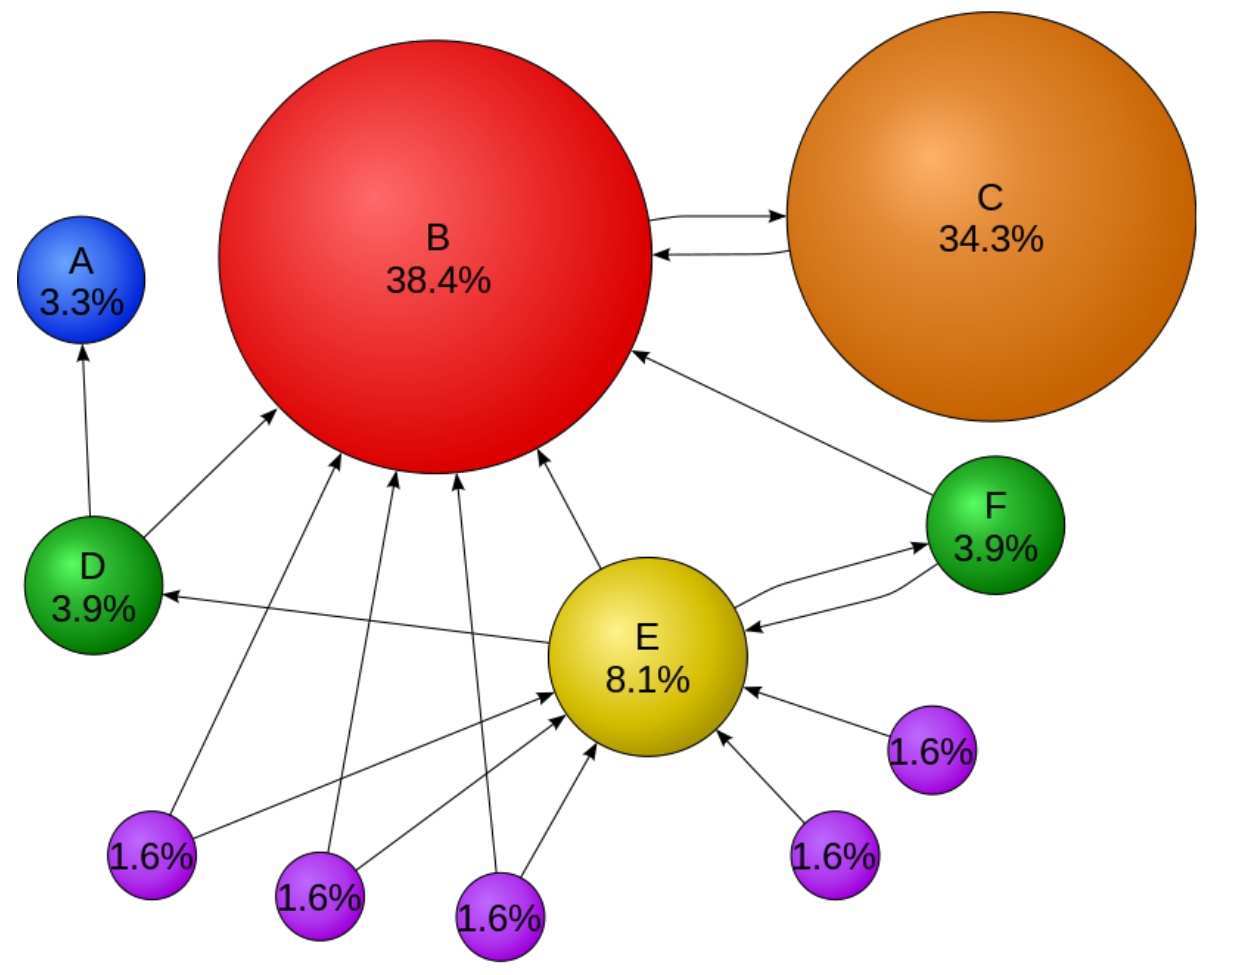
\includegraphics[width=0.60\textwidth]{pagerankscheme}
\caption{Sch\'{e}ma d\'un set d'URLs}
\label{fig:pagerankscheme}
\end{center}
\end{figure}
~\\*

Et voici le principe de fonctionnement de PageRank. \\*

\begin{enumerate}
\begin{item}

\begin{equation*}
PR(u) = \sum\nolimits_{v \in B \textsubscript{u}} \frac{PR(v)}{L(v)}
\end{equation*}
~\\*

La valeur du PageRank pour une page \textit{u} d\'{e}pend des valeurs du PageRank pour chaque page \textit{v} contenue dans l'ensemble \textit{B\textsubscript{u}} (l'ensemble contenant toutes les pages li\'{e}es \`{a} la page \textit{u}), divis\'{e} par le nombre L(v) de liens de la page \textit{v}. \\*

\end{item}
\begin{item}

L'algorithme it\'{e}ratif est le suivant : \\*

A \textit{t = 0}, une distribution de probabilit\'{e} est initialis\'{e}e de la sorte : \\*

\begin{equation*}
PR(p\textsubscript{i};0) = \frac{1}{N}
\end{equation*}
~\\*

\end{item}
\begin{item}

A chaque \'{e}tape \textit{t}, voici comment est calcul\'{e}e la nouvelle valeur du PageRank pour chaque page : \\*

\begin{equation*}
PR(p\textsubscript{i};t + 1) = \frac{1-d}{N} + d \sum\nolimits_{p\textsubscript{j} \in M(p\textsubscript{j})} \frac{PR(p\textsubscript{i};t)}{L(p\textsubscript{j})}
\end{equation*}
~\\*
\end{item}
\end{enumerate}

Pour des raisons de pr\'{e}cision et de facilit\'{e} de code, nous avons d\'{e}cid\'{e} de tout multiplier par N. \\*
 
%----------------------------------------------------------------------------------------
%	SECTION 4
%----------------------------------------------------------------------------------------

\section{Impl\'{e}mentation de PageRank}

Nous avons \'{e}crit un script \textit{Scala} qui, \`{a} partir des fichiers d'exemple \textit{example\_ arcs} et \textit{example\_ index}, ainsi qu'un nombre d'it\'{e}rations, calcule le PageRank de chacune des pages recens\'{e}es dans le second fichier.\\*

\begin{enumerate}
\begin{item}
R\'{e}cup\'{e}ration du nombre d'it\'{e}rations \`{a} r\'{e}aliser
\begin{tcolorbox}
\begin{lstlisting}[style=Scala]
val iters = if (args.length > 1) args(2).toInt else 10
\end{lstlisting}
\end{tcolorbox}
\end{item}
\begin{item}
R\'{e}cup\'{e}ration des arcs entre les diff\'{e}rentes URLs
\begin{tcolorbox}
\begin{lstlisting}[style=Scala]
val lines = spark.read.textFile(args(0)).rdd
val links = lines.map{ s =>
	val parts = s.split("\\s+")
	(parts(0), parts(1))
}.distinct().groupByKey().cache()
\end{lstlisting}
\end{tcolorbox}
\end{item}
\begin{item}
Assignation des poids initiaux aux diff\'{e}rents \'{e}l\'{e}ments
\begin{tcolorbox}
\begin{lstlisting}[style=Scala]
var ranks = links.mapValues(v => 1.0)
\end{lstlisting}
\end{tcolorbox}
\end{item}
\begin{item}
R\'{e}cup\'{e}ration des URLs dans l'ordre
\begin{tcolorbox}
\begin{lstlisting}[style=Scala]
val linesIndex = spark.read.textFile(args(1)).rdd
val index = linesIndex.map{ s =>
	val parts = s.split("\\s+")
	(parts(0))
}.distinct().cache()
val URLs = index.collect()
\end{lstlisting}
\end{tcolorbox}
\end{item}
\begin{item}
Calcul de chaque nouvelles valeurs du PageRank pour l'ensemble des it\'{e}rations
\begin{tcolorbox}
\begin{lstlisting}[style=Scala]
for (i <- 1 to iters) {
	val contribs = links.join(ranks).values.flatMap{ case (urls, rank) =>
		val size = urls.size
		urls.map(url => (url, rank / size))
	}
	ranks = contribs.reduceByKey(_ + _).mapValues(0.15 + 0.85 * _)
}
\end{lstlisting}
\end{tcolorbox}
\end{item}
\begin{item}
Affichage des r\'{e}sultats
\begin{tcolorbox}
\begin{lstlisting}[style=Scala]
val output = ranks.collect()
output.foreach{
	tup =>
	val element = URLs(tup._1.toInt)
	println(element + s" has rank:  ${tup._2}.")
}
\end{lstlisting}
\end{tcolorbox}
\end{item}
\end{enumerate}

%----------------------------------------------------------------------------------------
%	SECTION 5
%----------------------------------------------------------------------------------------

\section{R\'{e}sultats et bilan}

Voici une partie des r\'{e}sultats lorsqu'on lance le script avec les fichiers exemples. \\*

\begin{figure}[h]
\begin{center}
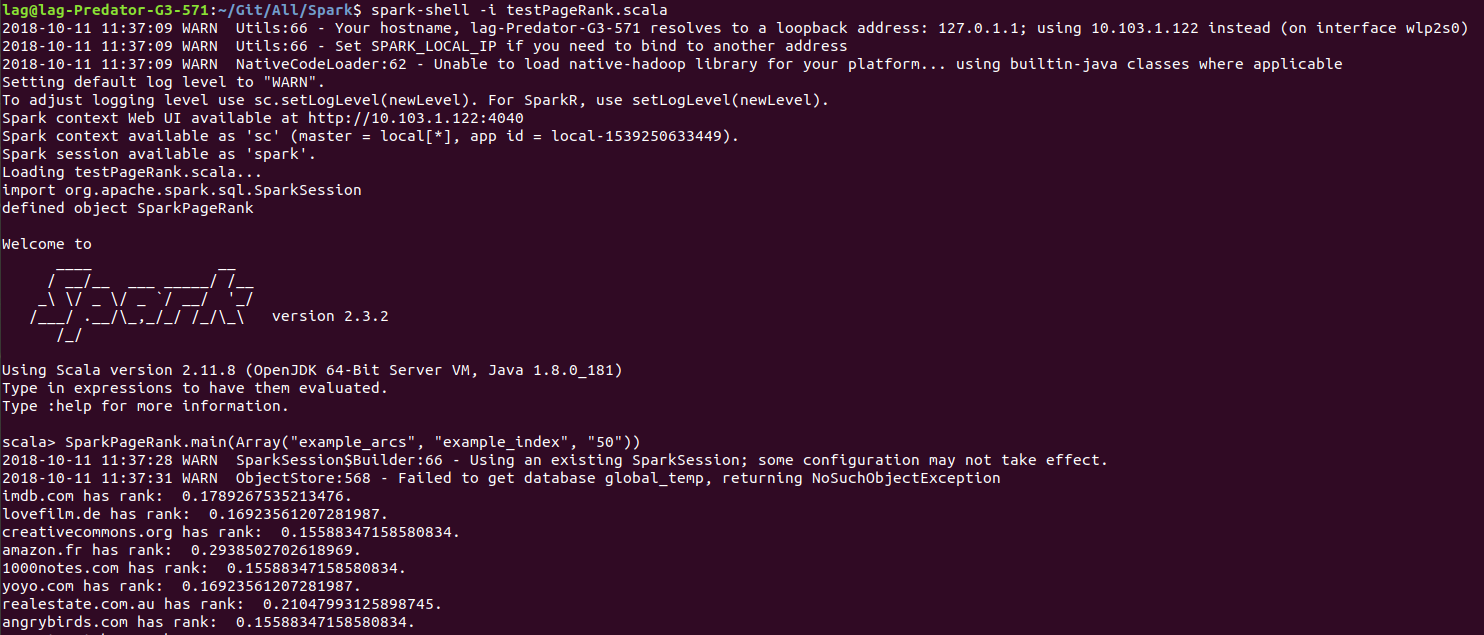
\includegraphics[width=0.60\textwidth]{results}
\caption{R\'{e}sultats de notre PageRank}
\label{fig:results}
\end{center}
\end{figure}
~\\*

Les r\'{e}sultats semblent concluants, en effet, "\`{a} la main", on constate que les pages qui poss\`{e}dent le plus d'entr\'{e}es sont le plus susceptible d'\^{e}tre visit\'{e}es, et vice-versa. PageRank est donc un puissant outil, et nous comprennons le principe de fonctionnement des moteurs de recherche tels que \textit{Google} ou \textit{Ecosia}.

\end{document}